\chapter*{Experiment 2 - Button}
\addcontentsline{toc}{chapter}{Experiment 2 - Button}
We wire up the experiment as shown in the diagram fig:~\ref{fig:exp2_button}. And upload the sketch code in the next section on page:~\pageref{sketch:exp2}.

%
\begin{figure}[ht]
	\centering
	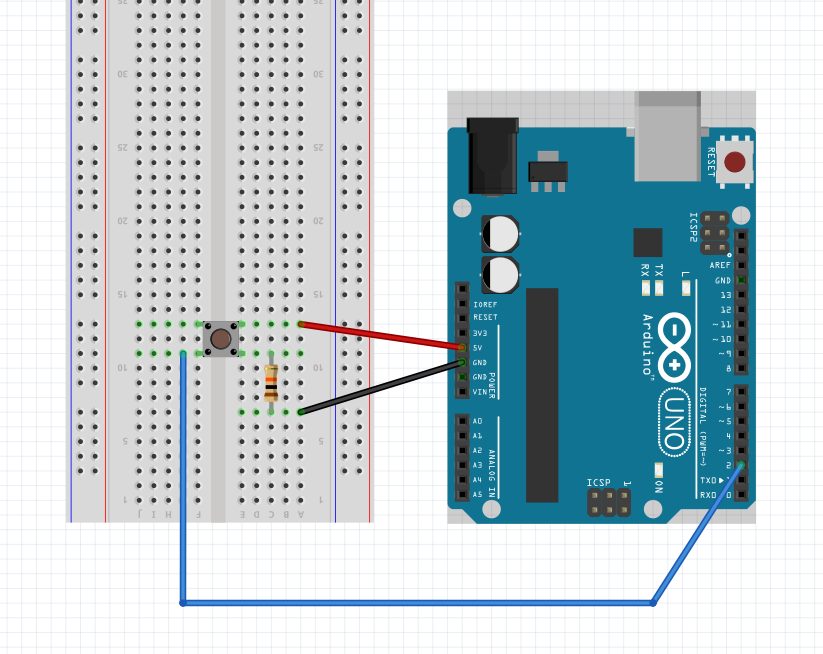
\includegraphics[width=12cm]{images/08}
	\caption{Read a buttons input \citep{fritzing-15}}
	\label{fig:exp2_button}
\end{figure}
%

Open the \textit{serial monitor} inside the \gls{Arduino} IDE, every second a 0 should be printed in the console window. When the button is pressed, a 1 will be printed instead.

\newpage
\section*{Sketch Code}
\label{sketch:exp2}
\begin{lstlisting}
/*
DigitalReadSerial
Reads a digital input on pin 2, prints the result to the serial monitor

This example code is in the public domain.
*/

// digital pin 2 has a pushbutton attached to it. Give it a name:
int pushButton = 2;
int buttonState;

// the setup routine runs once when you press reset:
void setup() {
  // initialize serial communication at 9600 bits per second:
  Serial.begin(9600);
  // make the pushbutton's pin an input:
  pinMode(pushButton, INPUT);
}

// the loop routine runs over and over again forever:
void loop() {
  // read the input pin:
  buttonState = digitalRead(pushButton);
  // print out the state of the button:
  Serial.println(buttonState);
  // delay in between reads for stability
  delay(100);
}
\end{lstlisting}